% Options for packages loaded elsewhere
\PassOptionsToPackage{unicode}{hyperref}
\PassOptionsToPackage{hyphens}{url}
%
\documentclass[
  14pt,
  ignorenonframetext,
  aspectratio=169,
]{beamer}
\usepackage{pgfpages}
\setbeamertemplate{caption}[numbered]
\setbeamertemplate{caption label separator}{: }
\setbeamercolor{caption name}{fg=normal text.fg}
\beamertemplatenavigationsymbolsempty
% Prevent slide breaks in the middle of a paragraph
\widowpenalties 1 10000
\raggedbottom

\usepackage{amsmath,amssymb}
\usepackage{iftex}
\ifPDFTeX
  \usepackage[T1]{fontenc}
  \usepackage[utf8]{inputenc}
  \usepackage{textcomp} % provide euro and other symbols
\else % if luatex or xetex
  \usepackage{unicode-math}
  \defaultfontfeatures{Scale=MatchLowercase}
  \defaultfontfeatures[\rmfamily]{Ligatures=TeX,Scale=1}
\fi
\usepackage{lmodern}
\ifPDFTeX\else  
    % xetex/luatex font selection
\fi
% Use upquote if available, for straight quotes in verbatim environments
\IfFileExists{upquote.sty}{\usepackage{upquote}}{}
\IfFileExists{microtype.sty}{% use microtype if available
  \usepackage[]{microtype}
  \UseMicrotypeSet[protrusion]{basicmath} % disable protrusion for tt fonts
}{}
\makeatletter
\@ifundefined{KOMAClassName}{% if non-KOMA class
  \IfFileExists{parskip.sty}{%
    \usepackage{parskip}
  }{% else
    \setlength{\parindent}{0pt}
    \setlength{\parskip}{6pt plus 2pt minus 1pt}}
}{% if KOMA class
  \KOMAoptions{parskip=half}}
\makeatother
\usepackage{xcolor}
\newif\ifbibliography
\setlength{\emergencystretch}{3em} % prevent overfull lines
\setcounter{secnumdepth}{-\maxdimen} % remove section numbering

\usepackage{color}
\usepackage{fancyvrb}
\newcommand{\VerbBar}{|}
\newcommand{\VERB}{\Verb[commandchars=\\\{\}]}
\DefineVerbatimEnvironment{Highlighting}{Verbatim}{commandchars=\\\{\}}
% Add ',fontsize=\small' for more characters per line
\usepackage{framed}
\definecolor{shadecolor}{RGB}{241,243,245}
\newenvironment{Shaded}{\begin{snugshade}}{\end{snugshade}}
\newcommand{\AlertTok}[1]{\textcolor[rgb]{0.68,0.00,0.00}{#1}}
\newcommand{\AnnotationTok}[1]{\textcolor[rgb]{0.37,0.37,0.37}{#1}}
\newcommand{\AttributeTok}[1]{\textcolor[rgb]{0.40,0.45,0.13}{#1}}
\newcommand{\BaseNTok}[1]{\textcolor[rgb]{0.68,0.00,0.00}{#1}}
\newcommand{\BuiltInTok}[1]{\textcolor[rgb]{0.00,0.23,0.31}{#1}}
\newcommand{\CharTok}[1]{\textcolor[rgb]{0.13,0.47,0.30}{#1}}
\newcommand{\CommentTok}[1]{\textcolor[rgb]{0.37,0.37,0.37}{#1}}
\newcommand{\CommentVarTok}[1]{\textcolor[rgb]{0.37,0.37,0.37}{\textit{#1}}}
\newcommand{\ConstantTok}[1]{\textcolor[rgb]{0.56,0.35,0.01}{#1}}
\newcommand{\ControlFlowTok}[1]{\textcolor[rgb]{0.00,0.23,0.31}{#1}}
\newcommand{\DataTypeTok}[1]{\textcolor[rgb]{0.68,0.00,0.00}{#1}}
\newcommand{\DecValTok}[1]{\textcolor[rgb]{0.68,0.00,0.00}{#1}}
\newcommand{\DocumentationTok}[1]{\textcolor[rgb]{0.37,0.37,0.37}{\textit{#1}}}
\newcommand{\ErrorTok}[1]{\textcolor[rgb]{0.68,0.00,0.00}{#1}}
\newcommand{\ExtensionTok}[1]{\textcolor[rgb]{0.00,0.23,0.31}{#1}}
\newcommand{\FloatTok}[1]{\textcolor[rgb]{0.68,0.00,0.00}{#1}}
\newcommand{\FunctionTok}[1]{\textcolor[rgb]{0.28,0.35,0.67}{#1}}
\newcommand{\ImportTok}[1]{\textcolor[rgb]{0.00,0.46,0.62}{#1}}
\newcommand{\InformationTok}[1]{\textcolor[rgb]{0.37,0.37,0.37}{#1}}
\newcommand{\KeywordTok}[1]{\textcolor[rgb]{0.00,0.23,0.31}{#1}}
\newcommand{\NormalTok}[1]{\textcolor[rgb]{0.00,0.23,0.31}{#1}}
\newcommand{\OperatorTok}[1]{\textcolor[rgb]{0.37,0.37,0.37}{#1}}
\newcommand{\OtherTok}[1]{\textcolor[rgb]{0.00,0.23,0.31}{#1}}
\newcommand{\PreprocessorTok}[1]{\textcolor[rgb]{0.68,0.00,0.00}{#1}}
\newcommand{\RegionMarkerTok}[1]{\textcolor[rgb]{0.00,0.23,0.31}{#1}}
\newcommand{\SpecialCharTok}[1]{\textcolor[rgb]{0.37,0.37,0.37}{#1}}
\newcommand{\SpecialStringTok}[1]{\textcolor[rgb]{0.13,0.47,0.30}{#1}}
\newcommand{\StringTok}[1]{\textcolor[rgb]{0.13,0.47,0.30}{#1}}
\newcommand{\VariableTok}[1]{\textcolor[rgb]{0.07,0.07,0.07}{#1}}
\newcommand{\VerbatimStringTok}[1]{\textcolor[rgb]{0.13,0.47,0.30}{#1}}
\newcommand{\WarningTok}[1]{\textcolor[rgb]{0.37,0.37,0.37}{\textit{#1}}}

\providecommand{\tightlist}{%
  \setlength{\itemsep}{0pt}\setlength{\parskip}{0pt}}\usepackage{longtable,booktabs,array}
\usepackage{calc} % for calculating minipage widths
\usepackage{caption}
% Make caption package work with longtable
\makeatletter
\def\fnum@table{\tablename~\thetable}
\makeatother
\usepackage{graphicx}
\makeatletter
\def\maxwidth{\ifdim\Gin@nat@width>\linewidth\linewidth\else\Gin@nat@width\fi}
\def\maxheight{\ifdim\Gin@nat@height>\textheight\textheight\else\Gin@nat@height\fi}
\makeatother
% Scale images if necessary, so that they will not overflow the page
% margins by default, and it is still possible to overwrite the defaults
% using explicit options in \includegraphics[width, height, ...]{}
\setkeys{Gin}{width=\maxwidth,height=\maxheight,keepaspectratio}
% Set default figure placement to htbp
\makeatletter
\def\fps@figure{htbp}
\makeatother

\makeatletter
\@ifpackageloaded{tcolorbox}{}{\usepackage[skins,breakable]{tcolorbox}}
\@ifpackageloaded{fontawesome5}{}{\usepackage{fontawesome5}}
\definecolor{quarto-callout-color}{HTML}{909090}
\definecolor{quarto-callout-note-color}{HTML}{0758E5}
\definecolor{quarto-callout-important-color}{HTML}{CC1914}
\definecolor{quarto-callout-warning-color}{HTML}{EB9113}
\definecolor{quarto-callout-tip-color}{HTML}{00A047}
\definecolor{quarto-callout-caution-color}{HTML}{FC5300}
\definecolor{quarto-callout-color-frame}{HTML}{acacac}
\definecolor{quarto-callout-note-color-frame}{HTML}{4582ec}
\definecolor{quarto-callout-important-color-frame}{HTML}{d9534f}
\definecolor{quarto-callout-warning-color-frame}{HTML}{f0ad4e}
\definecolor{quarto-callout-tip-color-frame}{HTML}{02b875}
\definecolor{quarto-callout-caution-color-frame}{HTML}{fd7e14}
\makeatother
\makeatletter
\@ifpackageloaded{caption}{}{\usepackage{caption}}
\AtBeginDocument{%
\ifdefined\contentsname
  \renewcommand*\contentsname{Table of contents}
\else
  \newcommand\contentsname{Table of contents}
\fi
\ifdefined\listfigurename
  \renewcommand*\listfigurename{List of Figures}
\else
  \newcommand\listfigurename{List of Figures}
\fi
\ifdefined\listtablename
  \renewcommand*\listtablename{List of Tables}
\else
  \newcommand\listtablename{List of Tables}
\fi
\ifdefined\figurename
  \renewcommand*\figurename{Figure}
\else
  \newcommand\figurename{Figure}
\fi
\ifdefined\tablename
  \renewcommand*\tablename{Table}
\else
  \newcommand\tablename{Table}
\fi
}
\@ifpackageloaded{float}{}{\usepackage{float}}
\floatstyle{ruled}
\@ifundefined{c@chapter}{\newfloat{codelisting}{h}{lop}}{\newfloat{codelisting}{h}{lop}[chapter]}
\floatname{codelisting}{Listing}
\newcommand*\listoflistings{\listof{codelisting}{List of Listings}}
\makeatother
\makeatletter
\makeatother
\makeatletter
\@ifpackageloaded{caption}{}{\usepackage{caption}}
\@ifpackageloaded{subcaption}{}{\usepackage{subcaption}}
\makeatother
\ifLuaTeX
  \usepackage{selnolig}  % disable illegal ligatures
\fi
\usepackage{bookmark}

\IfFileExists{xurl.sty}{\usepackage{xurl}}{} % add URL line breaks if available
\urlstyle{same} % disable monospaced font for URLs
\hypersetup{
  pdftitle={conmat: Programmatic generation of synthetic contact matrices},
  pdfauthor={M. J. Lydeamore},
  hidelinks,
  pdfcreator={LaTeX via pandoc}}

\usetheme{Monash}


% Monash title page
% One can alter the font size by setting eg 'titlefontsize: 20pt' in the YAML header
\setbeamerfont{title}{series=\bfseries,parent=structure,size=\fontsize{22}{28}}
\setbeamertemplate{title page}
{\placefig{-0.01}{-0.01}{width=1.01\paperwidth,height=1.01\paperheight}{bg-02.png}
\begin{textblock}{8.7}(1,2.8)\usebeamerfont{title}
{\color{black}\raggedright\par\inserttitle}
\end{textblock}
\begin{textblock}{8.7}(1,6.8)
{\color{black}\raggedright{\insertauthor}\mbox{}\\[0.2cm]
\insertdate}
\end{textblock}}


% Find images
\graphicspath{{_extensions/presentation/_images/background/}{_extensions/quarto-monash/presentation/_images/background/}{figs/}{figures/}{images/}{img/}}\title{\texttt{conmat}:
Programmatic generation of synthetic contact matrices}
\author{M. J. Lydeamore}
\date{22 September 2024}
\titlegraphic{
\includegraphics{bg-02.png}}

\begin{document}
\frame{\titlepage}

\begin{frame}{What are contact matrices}
\phantomsection\label{what-are-contact-matrices}
\end{frame}

\begin{frame}{Contact diary studies}
\phantomsection\label{contact-diary-studies}
Contact diary studies follow individuals and ask them:

\begin{itemize}
\tightlist
\item
  how many contacts of a certain type,
\item
  the duration of contact,
\item
  the location of the contact,
\item
  the frequency of the contact
\end{itemize}

They are undoubtedly the gold standard for data on the number of
contacts.

But they are prohibitively expensive, and logistically very challenging.
\end{frame}

\begin{frame}{POLYMOD}
\phantomsection\label{polymod}
Published in 2008, Mossong et. al undertook a contact diary study of
7290 participants across Europe.

\emph{It remains the most widely cited contact diary study}.

\begin{center}
\includegraphics{images/mossong-combined.png}
\end{center}
\end{frame}

\begin{frame}{Contact matrix projection}
\phantomsection\label{contact-matrix-projection}
Prem et. al formed a model that predicts the number of contacts based on
the age of participants.

This model then allows for prediction to settings that are outside the
original POLYMOD countries.
\end{frame}

\begin{frame}{What is provided:}
\phantomsection\label{what-is-provided}
\begin{columns}[T]
\begin{column}{0.5\textwidth}
\begin{center}
\includegraphics{images/prem-dir-mats.png}
\end{center}
\end{column}

\begin{column}{0.5\textwidth}
\begin{center}
\includegraphics{images/prem-spreadsheet.png}
\end{center}
\end{column}
\end{columns}
\end{frame}

\begin{frame}{Our model of contact}
\phantomsection\label{our-model-of-contact}
Not much information to train model. We use:

\[\begin{aligned}
c_{ij} = \beta_0 + \beta_1(|i-j|) + &\beta_2(|i-j|^2) + \beta_3(i\times j) + \beta_4(i+j) +\\ &\beta_5\max(i, j) + \beta_6\min(i, j)
\end{aligned}
\]

\begin{tcolorbox}[enhanced jigsaw, title=\textcolor{quarto-callout-tip-color}{\faLightbulb}\hspace{0.5em}{🤓 Akshually 🤓}, opacityback=0, opacitybacktitle=0.6, colbacktitle=quarto-callout-tip-color!10!white, bottomrule=.15mm, toprule=.15mm, toptitle=1mm, arc=.35mm, titlerule=0mm, colframe=quarto-callout-tip-color-frame, rightrule=.15mm, bottomtitle=1mm, leftrule=.75mm, coltitle=black, left=2mm, colback=white, breakable]

We want to fit this as a generalised additive model, so \emph{actually}
we have splines on these terms to satisfy the smoothness requirements.

This is very similar to the approach by Prem et. al who perform post-hoc
smoothing of the parameters after MCMC.

\end{tcolorbox}
\end{frame}

\begin{frame}{Model terms}
\phantomsection\label{model-terms}
\begin{center}
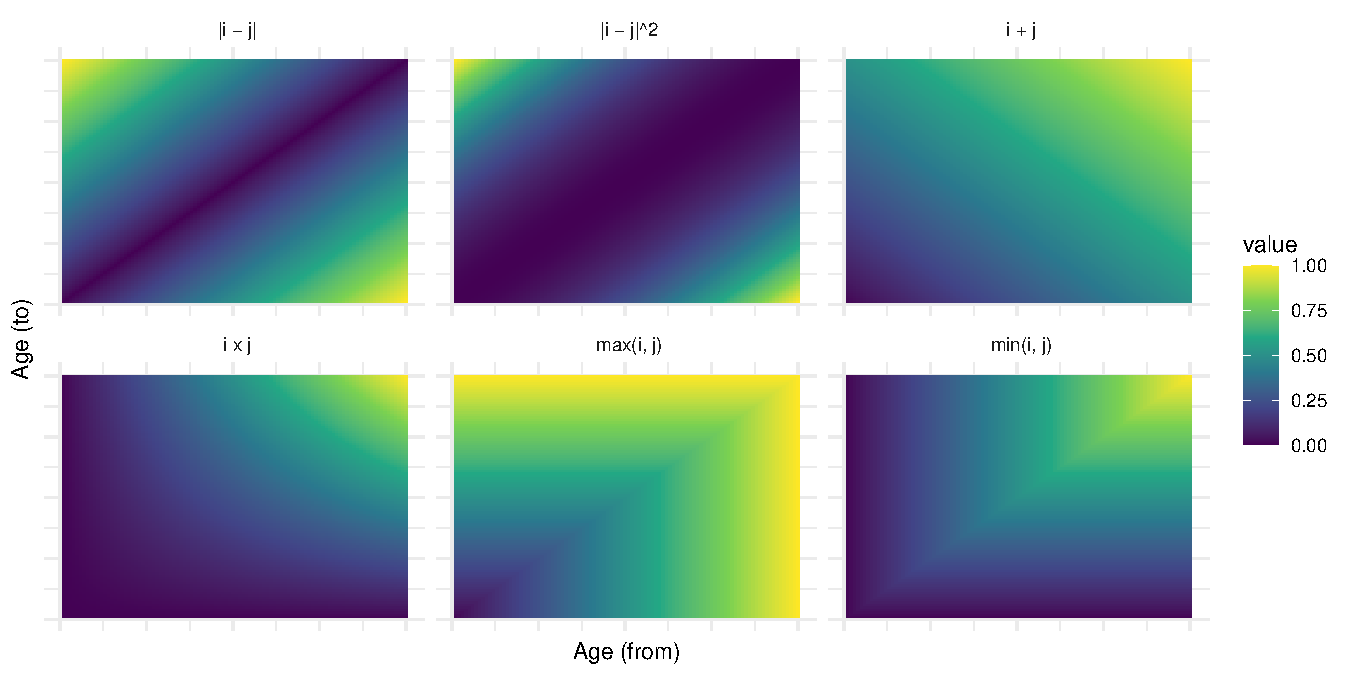
\includegraphics{index_files/figure-beamer/unnamed-chunk-3-1.pdf}
\end{center}
\end{frame}

\begin{frame}{Projection onto target demography}
\phantomsection\label{projection-onto-target-demography}
\begin{center}
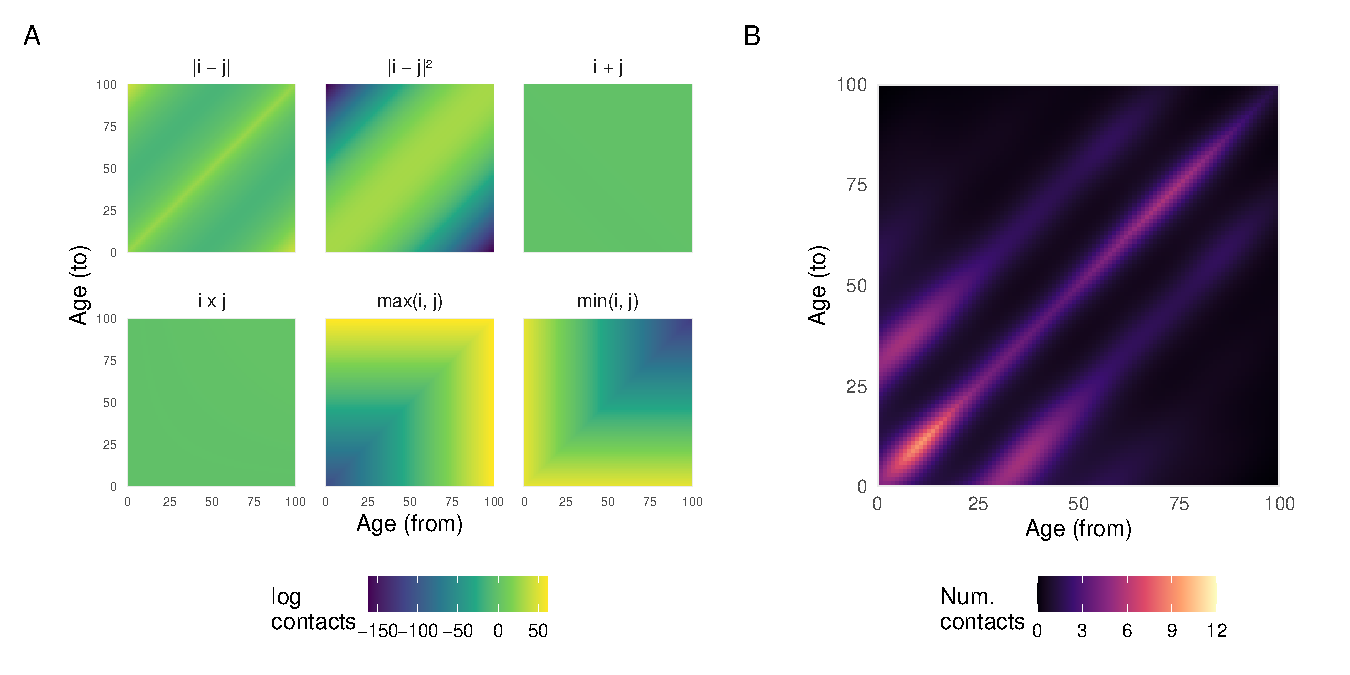
\includegraphics{index_files/figure-beamer/partial-plots-create-1.pdf}
\end{center}
\end{frame}

\begin{frame}[fragile]{Importance of contact diary study}
\phantomsection\label{importance-of-contact-diary-study}
We've used POLYMOD-trained models for over a decade.

There are 44 other surveys available in one collection on
\href{https://zenodo.org/communities/social_contact_data/records}{Zenodo},
and probably more out there in the wild.

Some recent work from \href{https://arxiv.org/abs/2406.01639}{Harris et.
al} has shown that differences in the survey design can have a
significant impact on these synthetic contact matrices.

\begin{tcolorbox}[enhanced jigsaw, title=\textcolor{quarto-callout-tip-color}{\faLightbulb}\hspace{0.5em}{Tip}, opacityback=0, opacitybacktitle=0.6, colbacktitle=quarto-callout-tip-color!10!white, bottomrule=.15mm, toprule=.15mm, toptitle=1mm, arc=.35mm, titlerule=0mm, colframe=quarto-callout-tip-color-frame, rightrule=.15mm, bottomtitle=1mm, leftrule=.75mm, coltitle=black, left=2mm, colback=white, breakable]

\texttt{conmat} allows for training on survey of choice, and projection
onto target demographic of choice

\end{tcolorbox}
\end{frame}

\begin{frame}[fragile]{Example of using a different study}
\phantomsection\label{example-of-using-a-different-study}
\begin{Shaded}
\begin{Highlighting}[]
\NormalTok{china\_survey }\OtherTok{\textless{}{-}}\NormalTok{ socialmixr}\SpecialCharTok{::}\FunctionTok{get\_survey}\NormalTok{(}\StringTok{"https://doi.org/10.5281/zenodo.3878754"}\NormalTok{) }\SpecialCharTok{|\textgreater{}}
    \FunctionTok{summarise}\NormalTok{(}\AttributeTok{contacts =} \FunctionTok{sum}\NormalTok{(cnt\_home))}

\NormalTok{china\_pop }\OtherTok{\textless{}{-}} \FunctionTok{read\_csv}\NormalTok{(}\StringTok{"./data/china\_pop\_age\_dist.csv"}\NormalTok{)}
\NormalTok{china\_pop\_cm }\OtherTok{\textless{}{-}}\NormalTok{ conmat}\SpecialCharTok{::}\FunctionTok{as\_conmat\_population}\NormalTok{(}
  \AttributeTok{data =}\NormalTok{ china\_pop,}
  \AttributeTok{age =}\NormalTok{ lower.age.limit,}
  \AttributeTok{population =}\NormalTok{ population}
\NormalTok{)}
\end{Highlighting}
\end{Shaded}
\end{frame}

\begin{frame}[fragile]{Example of using a different study}
\phantomsection\label{example-of-using-a-different-study-1}
\begin{Shaded}
\begin{Highlighting}[]
\NormalTok{china\_survey }\OtherTok{\textless{}{-}}\NormalTok{ socialmixr}\SpecialCharTok{::}\FunctionTok{get\_survey}\NormalTok{(}\StringTok{"https://doi.org/10.5281/zenodo.3878754"}\NormalTok{) }\SpecialCharTok{|\textgreater{}}
    \FunctionTok{summarise}\NormalTok{(}\AttributeTok{contacts =} \FunctionTok{sum}\NormalTok{(cnt\_home))}

\NormalTok{china\_pop }\OtherTok{\textless{}{-}} \FunctionTok{read\_csv}\NormalTok{(}\StringTok{"./data/china\_pop\_age\_dist.csv"}\NormalTok{)}
\NormalTok{china\_pop\_cm }\OtherTok{\textless{}{-}}\NormalTok{ conmat}\SpecialCharTok{::}\FunctionTok{as\_conmat\_population}\NormalTok{(}
  \AttributeTok{data =}\NormalTok{ china\_pop,}
  \AttributeTok{age =}\NormalTok{ lower.age.limit,}
  \AttributeTok{population =}\NormalTok{ population}
\NormalTok{)}

\NormalTok{model }\OtherTok{\textless{}{-}}\NormalTok{ conmat}\SpecialCharTok{::}\FunctionTok{fit\_single\_contact\_model}\NormalTok{(}
    \AttributeTok{contact\_data =}\NormalTok{ china\_survey,}
    \AttributeTok{population =}\NormalTok{ china\_pop\_cm}
\NormalTok{)}

\NormalTok{predicted\_contacts }\OtherTok{\textless{}{-}}\NormalTok{ conmat}\SpecialCharTok{::}\FunctionTok{predict\_contacts}\NormalTok{(}
    \AttributeTok{model =}\NormalTok{ model,}
    \AttributeTok{population =}\NormalTok{ china\_pop\_cm,}
    \AttributeTok{age\_breaks =} \FunctionTok{c}\NormalTok{(}\FunctionTok{seq}\NormalTok{(}\DecValTok{0}\NormalTok{, }\DecValTok{80}\NormalTok{, }\AttributeTok{by =} \DecValTok{5}\NormalTok{), }\ConstantTok{Inf}\NormalTok{)}
\NormalTok{)}
\end{Highlighting}
\end{Shaded}
\end{frame}

\begin{frame}{Why input survey matters}
\phantomsection\label{why-input-survey-matters}
These matrices are for a Chinese population, using a Chinese survey
(left) and POLYMOD (right), for the home setting.

\begin{center}
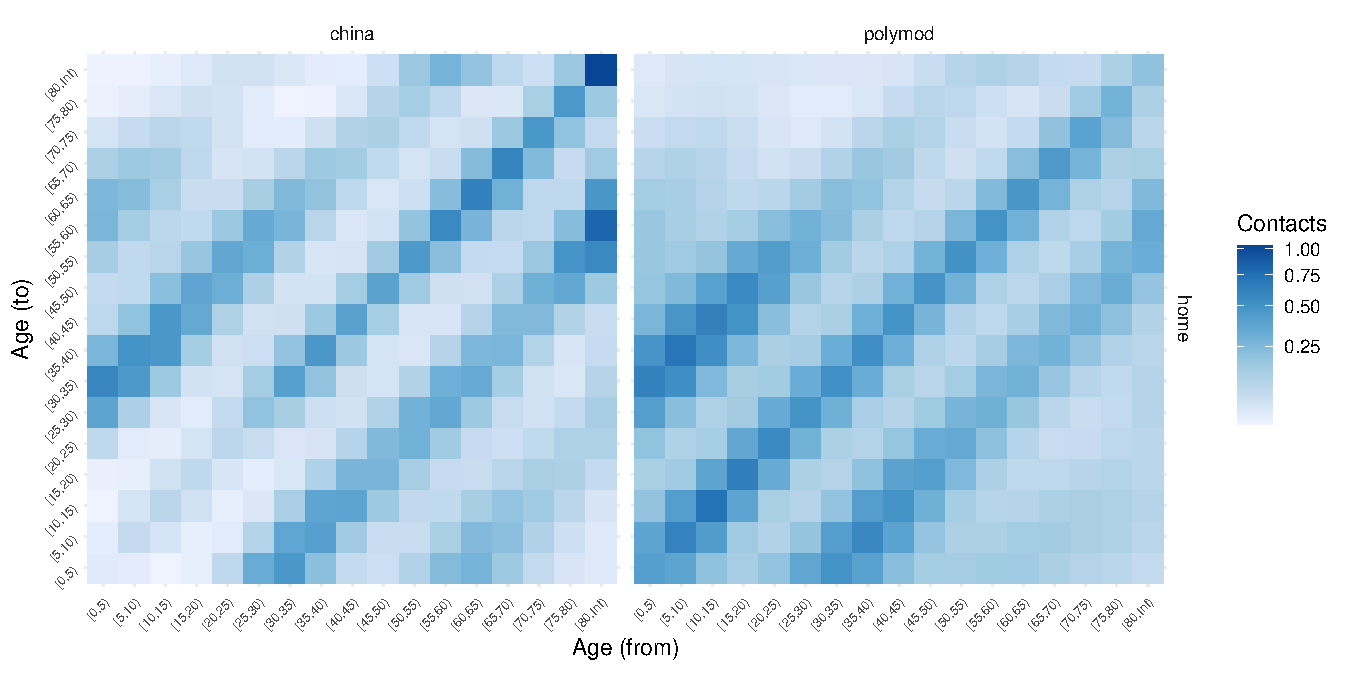
\includegraphics{index_files/figure-beamer/unnamed-chunk-7-1.pdf}
\end{center}
\end{frame}

\begin{frame}{Why input survey matters}
\phantomsection\label{why-input-survey-matters-1}
These matrices are for a Chinese population, using a Chinese survey
(left) and POLYMOD (right), for the home setting.

\begin{center}
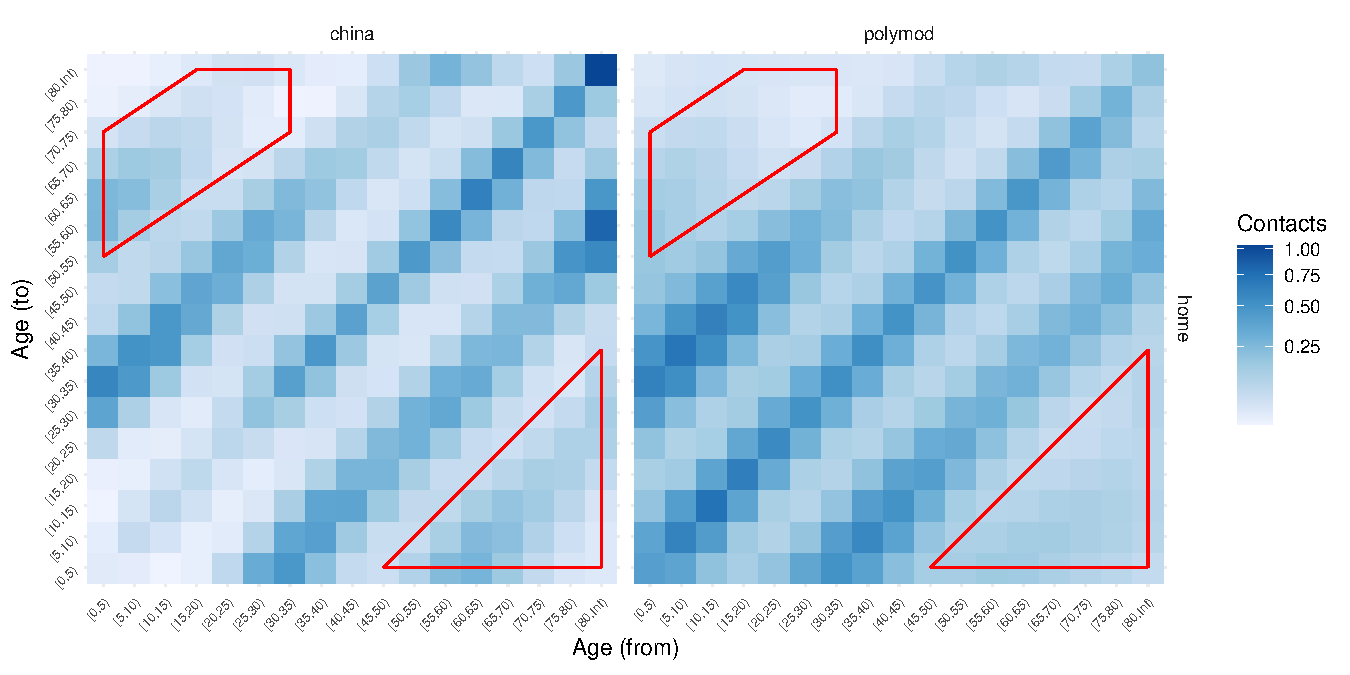
\includegraphics{index_files/figure-beamer/unnamed-chunk-8-1.pdf}
\end{center}
\end{frame}

\begin{frame}[fragile]{Summary}
\phantomsection\label{summary}
\texttt{conmat} is a new, open-source, programmable system to generate
synthetic contact matrices

\begin{itemize}[<+->]
\tightlist
\item
  Can use arbitrary contact survey and arbitrary demography
\item
  Convenience functions for next generation matrices, numbers of
  contacts
\item
  Choice of input survey \emph{is crucial}:

  \begin{itemize}[<+->]
  \tightlist
  \item
    These models have no information on terms like ``intergenerational
    mixing''
  \end{itemize}
\end{itemize}
\end{frame}

\begin{frame}[fragile]{Summary}
\phantomsection\label{summary-1}
\texttt{conmat} is a new, open-source, programmable system to generate
synthetic contact matrices

Available right now:

\begin{Shaded}
\begin{Highlighting}[]
\NormalTok{remotes}\SpecialCharTok{::}\FunctionTok{install\_github}\NormalTok{(}\StringTok{"idem{-}lab/conmat"}\NormalTok{)}
\end{Highlighting}
\end{Shaded}

or pre-computed matrices on Zenodo:
\url{https://zenodo.org/records/12776714}
\end{frame}

\begin{frame}{Acknowledgements}
\phantomsection\label{acknowledgements}
\begin{figure}

\begin{minipage}{0.25\linewidth}

\includegraphics{images/chitra-saraswati.png}

\subcaption{\label{}Chitra Saraswati}
\end{minipage}%
%
\begin{minipage}{0.25\linewidth}

\includegraphics{images/aarathy-babu.jpg}

\subcaption{\label{}Aarathy Babu}
\end{minipage}%
%
\begin{minipage}{0.25\linewidth}

\includegraphics{images/nick-tierney.jpg}

\subcaption{\label{}Nick Tierney}
\end{minipage}%
%
\begin{minipage}{0.25\linewidth}

\includegraphics{images/nick-golding.jpg}

\subcaption{\label{}Nick Golding}
\end{minipage}%

\end{figure}%

SPECTRUM-SPARK Seed Funding
\end{frame}



\end{document}
